% Create a Table of Contents in Beamer
\documentclass{beamer}
% Theme choice:
\usetheme{Singapore}
\usecolortheme{whale}
\setbeamercolor{titlelike}{fg=blue,bg=white}
\setbeamercolor{frametitle}{fg=blue,bg=white}
\setbeamertemplate{frametitle}[default][left]
\setbeamertemplate{navigation symbols}{}

\usepackage{graphicx}
\usepackage{amsmath}
\usepackage{amsfonts}
\usepackage{amssymb}
\usepackage{amsthm}

% Title page details: 
\title{Chapter 2: Regression for binary outcomes} 
\author{Taylor Okonek \& Charlie Wolock}
\date{\today}



\begin{document}
	% Title page frame
	\begin{frame}
	\titlepage 
\end{frame}

\begin{frame}{Learning objectives}
	By the end of Chapter 2, you should be able to: 
	\begin{itemize}
		\item Distinguish between probability and odds and know how to calculate each in \texttt{R}
		\item Describe the measures of association used for binary outcomes and exposures of interest
		\item Formulate a regression model, given a scientific or statistical question about a binary outcome
		\item Interpret the coefficients (along with confidence intervals and p-values) of a regression model for a binary outcome
		\item Describe how (and why) logistic regression interpretation changes when we have data from a case-control study
		\item Use \texttt{R} to fit a logistic regression model and produce supporting figures/tables
	\end{itemize}
\end{frame}

% Outline frame
\begin{frame}{Outline}
\tableofcontents
\end{frame}

\AtBeginSection[ ]
{
\begin{frame}{Outline}
\tableofcontents[currentsection]
\end{frame}
}

% Presentation structure
\section{Binary outcomes}

% quantitative outcomes from ch1
\begin{frame}{Recall: Variable type}
	In Chapter 1, we ask scientific questions involving quantitative outcomes: those that have a fundamentally numeric quality: 
	\\~\
	
	\textcolor{red}{Insert examples from Chapter 1.}
\end{frame}

% binary variable examples
\begin{frame}{Recall: Variable type}
Binary variables are a type of \textcolor{blue}{categorical} variable with two possible categories. We often implicitly think of them in a 0-1 sense, but they don't have actual numeric value. 
\\~\

Examples we often see in biomedical research: 
\begin{itemize}
	\item Type I diabetes (presence/absence)
	\item Surgery complications (occurred/did not occur)
	\item Smoking (yes/no)
	\item Mortality prior to age 5 (occurred/did not occur)
	\item COVID status (positive/negative)
\end{itemize}
\end{frame}

% binary variable scientific questions
\begin{frame}{Scientific questions about binary variables}
	Questions we could ask about these variables include
	\begin{itemize}
		\item Are variants in the HLA-DRB1 gene associated with \textcolor{blue}{Type I diabetes}? 
		\item Are \textcolor{blue}{surgery complications} after upper endoscopy associated with who (anesthesiologist vs nurse) performed the sedation?
		\item Is the use of e-cigarettes associated with \textcolor{blue}{smoking}?
		\item \textcolor{red}{Insert question from Taylor here}
		\item Is Vitamin D intake associated with the risk of \textcolor{blue}{testing positive for COVID}?
	\end{itemize}
\end{frame}

%\begin{frame}{Instructors}
%
%\begin{figure}
%	\begin{center}
%		
\includegraphics[height=0.4\textheight]{charlie.jpg} 
%		\hspace{2cm}
%		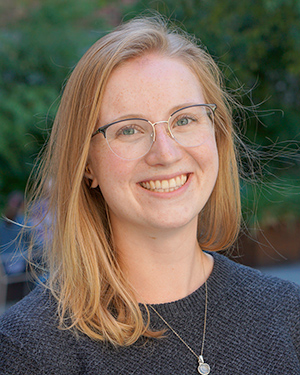
\includegraphics[height=0.4\textheight]{taylor.jpg}
%	\end{center}
%\end{figure}
%
%\begin{columns}
%	\begin{column}[t]{0.4\textwidth}
%            \small Charlie Wolock (he/him) \\~\
%            
%            \small 4th year Ph.D. Student, Dept. of Biostatistics
%            \small Statistical interests: Nonparametrics, survival analysis
%	\end{column}
%	\begin{column}[t]{0.4\textwidth}  %%<--- here
%			\small Taylor Okonek (she/her) \\~\ 
%			
%			\small 4th year Ph.D. Student, Dept. of Biostatistics
%			\small Statistical interests: spatial stats, infectious disease
%	\end{column}
%\end{columns}
%
%\end{frame}


\section*{References}
\begin{frame}
% to enforce entries in the table of contents
\end{frame}

\end{document}